% The forecast head (Section "Forecast head"). Build: pdflatex head_block.tex
% Checked against TransformerQuantileForecastingHead, src/forecasting_head.py
% at 6674dc92: pre-norm nn.TransformerEncoderLayer (GELU, FFN 4 d_model,
% dropout 0.1), 2 layers, a final LayerNorm, then one linear map to
% 9 quantiles x W values. At d_model = 64 this gives 109,456 parameters.
% Colours as in arch_block.tex; the output map is grey.
\documentclass[tikz,border=1pt]{standalone}
\usepackage[T1]{fontenc}
\usepackage{amsmath}
\usetikzlibrary{positioning,arrows.meta,fit,calc}
\definecolor{cnorm}{HTML}{F7F097}  % normalisation: yellow
\definecolor{cattn}{HTML}{F1CA73}  % attention: orange
\definecolor{cffn}{HTML}{A2D6F3}   % feed-forward: sky blue
\definecolor{clin}{HTML}{DDDDDD}   % output map: grey
\begin{document}
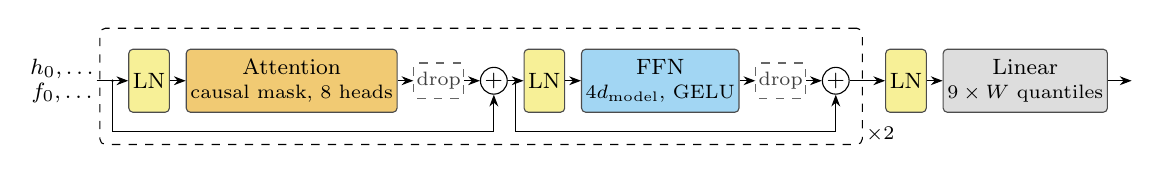
\begin{tikzpicture}[
  font=\footnotesize,
  node distance=2mm,
  box/.style={draw=black!70, rounded corners=1.5pt, align=center, inner sep=1.5pt,
    minimum height=8mm},
  op/.style={draw, circle, inner sep=0pt, minimum size=3.4mm},
  arr/.style={-{Stealth[length=1.5mm]}},
  drop/.style={draw=black!60, dashed, rounded corners=1pt, inner sep=1pt,
    font=\scriptsize, text=black!75, minimum height=4.5mm},
  note/.style={font=\scriptsize, text=black!60, align=center},
]
  \node[align=center, inner sep=1pt] (in) {$h_0, \ldots$\\[-1pt]$f_0, \ldots$};
  \node[box, fill=cnorm, right=4mm of in] (ln1) {LN};
  \node[box, fill=cattn, right=of ln1] (att) {Attention\\[-1pt]{\scriptsize causal mask, $8$ heads}};
  \node[drop, right=of att] (dp1) {drop};
  \node[op, right=of dp1] (add1) {$+$};
  \node[box, fill=cnorm, right=of add1] (ln2) {LN};
  \node[box, fill=cffn, right=of ln2] (ffn) {FFN\\[-1pt]{\scriptsize $4d_{\mathrm{model}}$, GELU}};
  \node[drop, right=of ffn] (dp2) {drop};
  \node[op, right=of dp2] (add2) {$+$};
  \node[box, fill=cnorm, right=4.5mm of add2] (ln3) {LN};
  \node[box, fill=clin, right=of ln3] (lin) {Linear\\[-1pt]{\scriptsize $9 \times W$ quantiles}};
  \coordinate[right=3mm of lin] (out);

  \draw[arr] (in) -- (ln1);
  \foreach \a/\b in {ln1/att, att/dp1, dp1/add1, add1/ln2, ln2/ffn,
                     ffn/dp2, dp2/add2, add2/ln3, ln3/lin, lin/out}
    \draw[arr] (\a) -- (\b);

  \coordinate (s1) at ($(in.east)!0.5!(ln1.west)$);
  \draw[arr] (s1) -- ++(0, -6.5mm) -| (add1.south);
  \coordinate (s2) at ($(add1.east)!0.5!(ln2.west)$);
  \draw[arr] (s2) -- ++(0, -6.5mm) -| (add2.south);
  \fill (s1) circle (0.5pt);
  \fill (s2) circle (0.5pt);

  \coordinate (lo) at ($(s1) + (0, -6.5mm)$);
  \coordinate (hi) at ($(att.north) + (0, 1mm)$);
  \node[draw, dashed, rounded corners=2pt, inner sep=1.6mm,
        fit=(ln1) (add2) (lo) (hi)] (blk) {};
  \node[note, anchor=south west, text=black, inner sep=1pt] at (blk.south east)
        {$\times 2$};
\end{tikzpicture}
\end{document}
